
\documentclass[a4paper,10pt]{article}
\usepackage{graphicx}
\usepackage{caption}
\usepackage{subcaption}

\graphicspath{ {./img/} }
\begin{document}

\title{\bf ISODS: An ISODATA-Based Initial Centroid Algorithm}
\author{Noah Gardner$^1$, Sahar Yarmohammadtoosky$^2$, \\
      Anthony Phan$^3$, and Chih-Cheng Hung$^4$\\[1ex]
      \sl \small Kennesaw State University, Marietta, GA, USA$^{1, 3, 4}$\\
      \sl \small Iran University of Science and Technology, Tehran,
      Iran$^2$\\[1ex]
      \small $^1$ngardn10@students.kennesaw.edu, \small
      $^2$yarmohamadishr@gmail.com, \\
      \small $^3$aphan5@students.kennesaw.edu, \small $^4$chung1@kennesaw.edu,
      \\}
\date{}
\maketitle

\begin{abstract}
      \noindent 
      Iterative Self-Organizing Data Analysis Technique (ISODATA) is a
      clustering algorithm based on K-Means that intends to find the correct
      number of clusters through merging and splitting. Compared to K-Means, the
      ISODATA algorithm should be resilient to initial cluster centers. However,
      ISODATA is also sensitive to initial cluster centers which impacts the
      performance of the algorithm. This work proposes using the ISODATA
      approach of splitting clusters to select quality initial cluster centers.
      The proposed approach is evaluated on several benchmark UCI datasets as
      well as the Salinas-A hyperspectral image dataset. The results are
      evaluated using standard clustering evaluation parameters. \\
      {\bf Keywords :} Clustering, ISODATA, Initial Centroids, Remote Sensing
\end{abstract}


% =========================================================================== %


\section{Introduction}

Remote sensing technology is used when the data collection takes place at a
remote distance from the subject matter, such as the study of daily weather and
long-term climate change, land cover monitoring, ecosystem modeling of
vegetation, and so on \cite{Jensen1996,Mallapragada2018}. Multispectral imaging
technology is one of the instruments for remote sensing used since the late
1960s \cite{Khan2018,Landgrebe1999}. However, multispectral imaging systems use
a low number of spectral bands (three to six spectral bands in different
systems). Increasing spectral resolution in the hyperspectral images (HSI) with
several hundred spectral bands of the observational scene in a single
acquisition makes it possible to acquire detailed examination of observational
scenes \cite{Khan2018}. The ground-based version of hyperspectral images has
gained immense interest. It has been applied to numerous electronic imaging
applications, including food inspection, forensic science, medical surgery and
diagnosis, and military applications
\cite{Govender2009,Adam2009,Fischer2006,Carrasco2003}. Because of the difficulty
of obtaining prior knowledge in remote sensing studies, unsupervised
classification and cluster analysis have great importance compared to supervised
classification \cite{Abbas2016}.

Unsupervised learning is a machine learning technique used when the learning
algorithm has no pre-existing labels and looks for patterns in the data set with
minimum human supervision and without external guidance. In contrast to
supervised learning, where a training set of inputs and observations are given
to the method, unsupervised learning uses only the inputs and should find an
interesting pattern in the data set. Two main approaches are used in
unsupervised learning, named principal component \cite{Mallapragada2018} and
cluster analysis \cite{Xu2015}. In the clustering method, unlabeled and unsorted
data points are grouped and segmented according to similarities and differences
to find structure in the inputs, group it into meaningful clusters, and
understand the data set better. There are different algorithms for Clustering,
such as K-Means, fuzzy C-Means, ISODATA \cite{Ball1965}, and so on. In the
K-Means algorithm, the goal is to minimize the sum of the squared distances
points have in the data set from its center. The problem with the K-Means
algorithm is that it requires a priori knowledge about the number of classes in
the data set, and choosing the cluster centers randomly may not result in
optimal partitioning of the data set.

One of the most popular clustering algorithms is called ISODATA clustering,
based on the K-means algorithm with some variations. The ISODATA method's
preference in comparison with the K-means algorithm is that the ISODATA
algorithm uses splitting and merging forms for clusters. The ISODATA method
allows starting from arbitrary cluster centers and obtains better partitioning
results than the K-Means algorithm, but it is not entirely resilient to initial
cluster centers. In this paper, a novel method using the ISODATA approach of
splitting clusters to select quality initial cluster centers is proposed.

The paper is organized as follows: Section 2 introduces K-Means and ISODATA
clustering algorithms. The new proposed algorithm is explained in Section 3. We
present the experimental results in Section 4. Finally, Section 5 contains
concluding remarks.

% =========================================================================== %

\section{Background}

\subsection{K-Means Algorithm}

The K-Means algorithm is an unsupervised clustering algorithm and aims to
partition $N$ observations into $K$ clusters [CITE]. Data points in the same
cluster are very similar to each other and have less variation compared to data
points assigned to other clusters. The user defines $K$, the number of expected
clusters. Following is a description of the K-Means algorithm:

\begin{itemize}
      \item \textbf{Step 1:} Choose $K$ cluster centers from the data set.
      \item \textbf{Step 2:} Assign each element of the data set to the cluster
            based on the minimum distance from the cluster center.
      \item \textbf{Step 3:} Re-calculate new cluster centers for each cluster
            after the assignment in \textbf{Step 2} by computing the mean of all
            patterns assigned to each cluster.
      \item \textbf{Step 4:} Repeat \textbf{Step 2 and Step 3} until clustering
            convergence occurs, or the set number of iterations is exceeded.
\end{itemize}

For selecting the initial cluster centers in \textbf{Step 1}, there are two
standard methods: Random Centers, and K-Means++ [CITE]. In Random Centers, $K$
samples are randomly chosen from the dataset to serve as the initial cluster
centers. In K-Means++, $1$ sample is randomly chosen from the dataset to serve
as the initial cluster center. Then, $K-1$ samples are iteratively selected,
where the probability of a sample being chosen as a cluster center is the
distance of the sample from previously chosen centers [CITE]. The K-Means
algorithm is susceptible to initial starting cluster centers, where different
initial values can result in a different classification.

\subsection{ISODATA Algorithm}

ISODATA is another frequently used clustering algorithm and is based on the
K-Means algorithm. Like K-Means, cluster centers are iteratively updated and
reassigned to the samples in the dataset. However, ISODATA determines the number
of clusters dynamically and allows for a different number of cluster centers. In
contrast, the K-Means algorithm requires a fixed user-set parameter of the
number of expected clusters. The advantage found within ISODATA allows for
discovery of a different number of clusters, which is achieved through
discarding clusters with a small number of member samples, and merging and
splitting clusters that meet certain parameters. There are three main ISODATA
parameters:

\begin{itemize}
      \item $\theta n$ - minimum number of cluster members, which determines
            whether the cluster is discarded,
      \item $\theta e$ - maximum standard deviation allowed for a cluster, which
            determines whether the cluster is split,
      \item $\theta c$ - minimum distance between clusters, which determines
            whether two clusters are merged.
\end{itemize}

Additionally, the user must set $K$, the maximum number of clusters to generate.
The ISODATA algorithm is briefly explained below:

\begin{itemize}
      \item \textbf{Step 1:} Choose $K$ cluster centers from the data set.
      \item \textbf{Step 2:} Assign each element of the dataset to the cluster
            based on the minimum distance from the cluster center.
      \item \textbf{Step 3:} Re-calculate new cluster centers for each cluster
            by computing the mean of all patterns assigned to each cluster.
      \item \textbf{Step 4:} Discard clusters that have fewer than ($\theta n$)
            members. If any clusters were discarded, move to \textbf{Step 7}.
      \item \textbf{Step 5:} If this iteration is an odd numbered iteration or
            the number of clusters is less than or equal to  $1/2 * K$, then
            split clusters which have a standard deviation in a dimension
            greater than ($\theta e$). Move to \textbf{Step 7}.
      \item \textbf{Step 6:} If this iteration is an even numbered iteration or
            the number of clusters is greater than or equal to $2 * K$, then
            merge clusters which have an intercluster distance less than
            ($\theta c$).
      \item \textbf{Step 7:} If this is not the last iteration, start the
            process again at step 2. If this is the last iteration or clustering
            convergence occurs, then end the process.
\end{itemize}

There are some disadvantages to the ISODATA algorithm. First, it is sensitive to
the parameters $\theta n$, $\theta e$, and $\theta c$. These parameters should
be fine-tuned for optimal performance based on the attributes of the dataset
being tested. In addition, similar to K-Means, it is sensitive to initial
cluster centers, although less so than K-Means due to the extra processes of
discarding, splitting, and merging. The initial centroids can affect both the
quality of clusters produced and the number of iterations required to converge
      [CITE].

% =========================================================================== %

\section{Proposed Method}

The proposed clustering algorithm's objective is to improve the result we obtain
from the clustering algorithms by targeting the initial cluster centers.
Inspired by the ISODATA algorithm, Iterative Self-Organizing Data Split (ISODS)
uses the splitting process from ISODATA to create the required initial cluster
centers to use for a clustering algorithm. The inputs for the algorithm are the
number of cluster centers $K$ as an integer, and the data to generate centers
from. 

The algorithm starts by selecting $1$ sample as an initial cluster center. In
the next step, each data is assigned to the cluster and the mean of the cluster
is updated. Then, by the ISODATA splitting process, each cluster is split along
the dimension with the highest standard deviation. The assignments for the new
clusters are calculated based on distance and the centers are updated. This
process is continued until either the number of clusters is greater than or
equal to $K$. If the number of clusters is greater than $K$, the clusters with
the fewest members are discarded one at a time, and the assignments and centers
are updated after each rejection. The algorithm is outlined below:

\begin{itemize}
      \item \textbf{Step 1:} Choose $1$ observation as a cluster center from the
            dataset.
      \item \textbf{Step 2:} Assign each element of the dataset to the cluster
            based on the minimum distance from the cluster center.
      \item \textbf{Step 3:} Re-calculate new cluster centers for each cluster
            by computing the mean of all patterns assigned to each cluster.
      \item \textbf{Step 4:} If the number of clusters is equal to $K$, then the
            process is terminated. If the number of clusters is greater than
            $K$, then the clusters with the fewest members is discarded, and the
            algorithm moves to \textbf{Step 2}.
      \item \textbf{Step 5:} Calculate the standard deviation of each cluster in
            each dimension. Then, split each cluster along the dimension with
            the greatest standard deviation.
\end{itemize}

This method began as a modified ISODATA process. However, the modification was
unique in that there is a clear distinction from the proposed change and the
beginning of the original process. Although more complex than other methods of
generating initial cluster centers, this approach guarantees variance between
clusters. As a result, ISODS can be used to generate clusters for other
clustering algorithms, such as K-Means.

% =========================================================================== %

\begin{table}[ht]
      \begin{tabular}{ |p{1.25cm}||p{1.25cm} p{1.25cm} p{1.25cm} p{1.25cm} p{1.25cm} p{1.25cm}|}
            \hline
            \multicolumn{7}{|c|}{\textbf{ISODATA}}                               \\
            \hline
            Init. & Iter.  & Clusters & ARI             & RI    & MI    & HI     \\
            \hline
            \multicolumn{7}{|c|}{\textit{Iris}}                                  \\[1ex]
            ISODS & 13.46  & 2.599    & \textbf{0.646}  & 0.826 & 0.173 & 0.653  \\
            KM++  & 15.43  & 2.544    & 0.628           & 0.816 & 0.184 & 0.631  \\
            Rand  & 11.90  & 2.41     & 0.607           & 0.802 & 0.198 & 0.604  \\
            \hline
            \multicolumn{7}{|c|}{\textit{Glass (Normalized)}}                    \\[1ex]
            ISODS & 3.19   & 1.066    & \textbf{0.0018} & 0.266 & 0.734 & -0.468 \\
            KM++  & 4.02   & 1.028    & 0.0011          & 0.265 & 0.735 & -0.470 \\
            Rand  & 3.69   & 1.055    & 0.0013          & 0.266 & 0.733 & -0.467 \\
            \hline
            \multicolumn{7}{|c|}{\textit{Wine}}                                  \\[1ex]
            ISODS & 9.16   & 1.836    & \textbf{0.313}  & 0.618 & 0.382 & 0.236  \\
            KM++  & 8.76   & 1.816    & 0.307           & 0.612 & 0.388 & 0.224  \\
            Rand  & 9.26   & 1.810    & 0.304           & 0.608 & 0.391 & 0.217  \\
            \hline 
            \multicolumn{7}{|c|}{\textbf{K-Means}}                               \\
            \hline
            \multicolumn{7}{|c|}{\textit{Iris}}                                  \\[1ex]
            ISODS & 2.29   & 3        & \textbf{0.623}  & 0.833 & 0.167 & 0.667  \\
            KM++  & 4.149  & 3        & 0.584           & 0.811 & 0.189 & 0.621  \\
            Rand  & 29.402 & 3        & 0.569           & 0.797 & 0.203 & 0.593  \\
            \hline
            \multicolumn{7}{|c|}{\textit{Glass (Normalized)}}                    \\[1ex]
            ISODS & 5.651  & 6        & 0.164           & 0.665 & 0.335 & 0.329  \\
            KM++  & 4.866  & 6        & \textbf{0.173}  & 0.643 & 0.357 & 0.285  \\
            Rand  & 77.178 & 6        & 0.151           & 0.634 & 0.366 & 0.268  \\
            \hline
            \multicolumn{7}{|c|}{\textit{Wine}}                                  \\[1ex]
            ISODS & 3.145  & 3        & \textbf{0.882}  & 0.947 & 0.053 & 0.895  \\
            KM++  & 5.388  & 3        & 0.839           & 0.926 & 0.074 & 0.851  \\
            Rand  & 24.775 & 3        & 0.834           & 0.920 & 0.080 & 0.840  \\
            \hline
      \end{tabular}
      \caption{UCI benchmark dataset results averaged over 1000 iterations of
            ISODATA and K-Means comparing three different initial cluster center
            algorithms (\textit{Init.}). Results in the table contain
            information on average iterations required (\textit{Iter.}), average
            number of clusters created (\textit{Clusters}), and validity
            measures.}
      \label{tab:ucitable}
\end{table}

\section{Results}

Due to the response of the ISODATA algorithm to the discarding, merging, and
splitting parameters, these parameters should be carefully selected. Since the
goal of this research is to explore the impact of initial cluster centers on
ISODATA, we use a relatively simple approach for generating ISODATA parameters.
Based on the available training data with included labels, each class is
summarized with the mean and standard deviation of that class, as well as the
number of members in each class. Typically, since we are working with
unsupervised learning algorithms, class information may not be available.

To determine $\theta n$, the minimum number of cluster members used for
discarding, we find the class with the fewest members and use the number of
members in that class as $\theta n$. For $\theta e$, the maximum standard
deviation allowed for a cluster, we follow a similar approach and find the
maximum standard deviation within a class. Finally, for $\theta c$, we calculate
the distance between the means of each class, and use the minimum distance as
$\theta c$. 

For the first experimental results shown in Table \ref{tab:ucitable}, we explore
applying ISODS to ISODATA and K-Means by using benchmark UCI \textit{Iris,}
\textit{Wine,} and \textit{Glass} datasets \cite{Dua2019}. We also show results
from applying Random Centers and K-Means++ Centers. For the \textit{Glass}
dataset, the data was Z-Score normalized (based on Z-Score of the training data)
because ISODATA can have problems converging on the raw dataset. We used $80\%$
of the data for training and $20\%$ of the data for testing to evaluate the
models. Following standard practice, the models were trained on the training
data, then fit to the test data. For the ISODATA parameters, we used the
approach of summarizing the class data based on the information in the training
data. The output labels (cluster assignments) were compared to the ground truth
labels contained in the test data using pair-counting measures. 

To evaluate the cluster results, external cluster validation measures are used.
We utilize pair-counting measures which rely on counting matching pairs between
two sets of data to determine agreement and disagreement \cite{Rezaei2016}. The
pair-counting measures applied are \textit{rand index} (RI - agreement
probability), \textit{adjusted rand index} (ARI), \textit{mirkin's index} (MI -
disagreement probability), and \textit{hubert's index} (HI - $(P(agree)$ -
$P(disagree))$) \cite{Hubert1985, Meila2003}. When comparing ground truth labels
to cluster assignments, RI can serve as an estimation of the accuracy. ARI is
similar to the RI, though it is corrected for chance and thus does not count
randomly generated labels \cite{Rand1971}.

\begin{figure}[ht]
      \centering
      \begin{subfigure}[b]{0.4\textwidth}
            \centering
            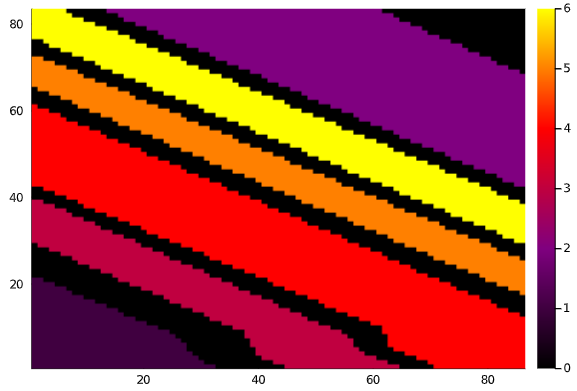
\includegraphics[width=\linewidth]{salinasgt.png}
            \caption{Salinas-A Ground Truth}
            \label{fig:salinasgt}
      \end{subfigure}
      \begin{subfigure}[b]{0.4\textwidth}
            \centering
            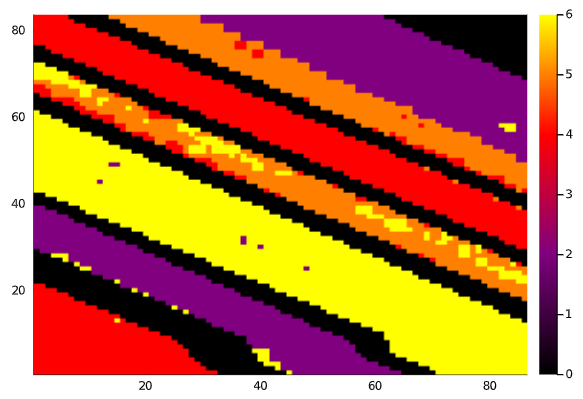
\includegraphics[width=\linewidth]{risodata.png}
            \caption{Random Centers (ARI=0.797)}
            \label{fig:salinasr}
      \end{subfigure}\hfill
      \centering
      \begin{subfigure}[b]{0.4\textwidth}
            \centering
            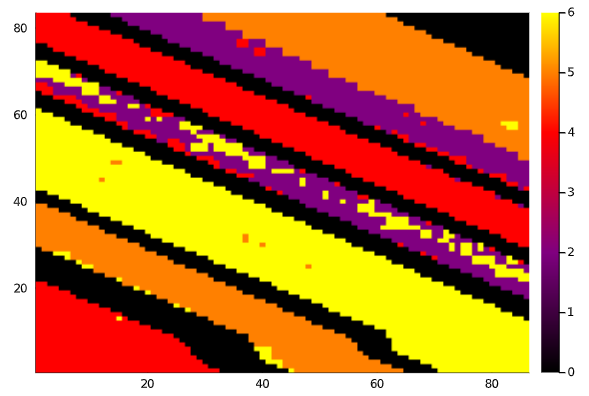
\includegraphics[width=\linewidth]{kisodata.png}
            \caption{KM++ Centers (ARI=0.781)}
            \label{fig:salinask}
      \end{subfigure}
      \begin{subfigure}[b]{0.4\textwidth}
            \centering
            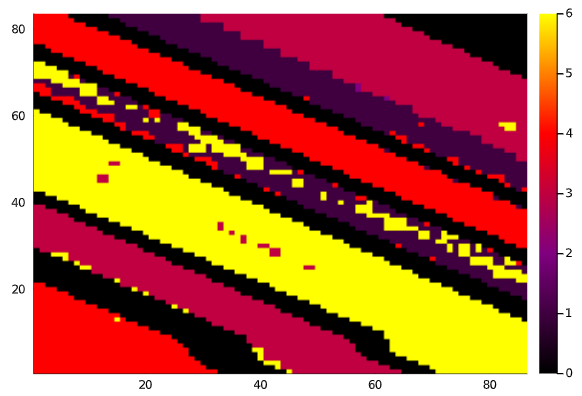
\includegraphics[width=\linewidth]{iisodata.png}
            \caption{ISODS Centers (ARI=0.758)}
            \label{fig:salinasi}
      \end{subfigure}\hfill \caption{Heatmap showing cluster assignments of each
            pixel using ISODATA with different initial cluster center methods.}
      \label{fig:salinas}
\end{figure}

Following the results on the benchmark datasets, we applied ISODATA to the
Salinas-A hyperspectral image dataset \cite{Salinas}. Salinas-A is a small
subscene of the Salinas image. It has a size of $86$ pixels by $83$ pixels, each
pixel contains $224$ bands, and each pixel is assigned to $1$ of $6$ classes,
disregarding the background. Due to the large number of dimensions in this
dataset, prinicipal component analysis (PCA) is used to extract features
\cite{Rodarmel2002}. In this experimental setup, we use $3$ prinicipal
components as the input to the model. We utilize the same 80/20 test-train split
as the previous experiment and Z-Score Normalize the data. Additionally, the
same ISODATA parameter selection approach is employed. Then, we run ISODATA for
$1000$ iterations using ISODS, K-Means++ Centers, and Random Centers. We save
the best performing model (based on test data performance) for each initial
cluster center approach and fit each pixel to the original dataset to obtain the
pictures shown in Figure \ref{fig:salinas}. Finally, the external cluster
validation measures are shown in Table \ref{tab:salinastable}. 

\begin{table}[ht]
      \begin{tabular}{ |p{1.25cm}||p{1.25cm} p{1.25cm} p{1.25cm} p{1.25cm} p{1.25cm} p{1.25cm}|}
            \hline
            \multicolumn{7}{|c|}{\textbf{ISODATA} - \textit{Salinas-A}}        \\
            \hline
            Init. & Iter. & Clusters & ARI            & RI    & MI    & HI     \\
            \hline
            \multicolumn{7}{|c|}{\textit{Average}}                             \\[1ex]
            ISODS & 2.772 & 2.42     & \textbf{0.156} & 0.388 & 0.612 & -0.224 \\
            KM++  & 3.177 & 1.097    & 0.019          & 0.228 & 0.772 & -0.544 \\
            Rand  & 3.693 & 1.584    & 0.084          & 0.308 & 0.691 & -0.383 \\
            \hline
            \multicolumn{7}{|c|}{\textit{Best}}                                \\[1ex]
            ISODS & 2     & 6        & 0.758          & 0.921 & 0.078 & 0.842  \\
            KM++  & 8     & 6        & 0.781          & 0.930 & 0.070 & 0.860  \\
            Rand  & 14    & 6        & \textbf{0.798} & 0.933 & 0.066 & 0.867  \\
            \hline
      \end{tabular}
      \caption{Salinas-A dataset average and best results over 1000 iterations
            of ISODATA comparing three different initial cluster center
            algorithms (\textit{Init.}). Results in the table contain
            information on iterations required (\textit{Iter.}), number of
            clusters created (\textit{Clusters}), and validity measures.}
      \label{tab:salinastable}
\end{table}

% =========================================================================== %

\section{Conclusion}
This study presents a method for generating initial cluster centers based on a
splitting approach, ISODS. We tested ISODS on bechmark datasets as well as the
Salinas-A hyperspectral image dataset. Both tests on average shows the
performance of ISODS using external cluster validation measures, especially on
the \textit{adjusted rand index} measure. Additonally, ISODS may decrease the
number of iterations required for a clustering algorithm such as ISODATA or
K-Means to converge. However, due to the complexity of the ISODS approach,
specifically calculating the means of the clusters, the number of iterations
taken by ISODS should be considered. When used in conjunction with ISODATA,
ISODS also shows an average number of clusters generated closer to the expected
output.

% =========================================================================== %

\subsection*{Acknowledgements}
This research was supported by the College of Computing and Software Engineering
at Kennesaw State University. We also want to thank our Laboratory for Machine
Vision and Security Research for providing us resources and mentoring.

\vspace{5mm}

\bibliographystyle{unsrt}
\bibliography{paper}

\end{document}
